\documentclass{article}
\usepackage[utf8]{inputenc}
\usepackage{graphicx}
\usepackage{biblatex}
\usepackage{tabularx}
\usepackage{graphicx}
\usepackage[table,xcdraw]{xcolor}
\usepackage{booktabs}

\addbibresource{bibliography.bib}
\newcommand{\beginsupplement}{%
        \setcounter{table}{0}
        \renewcommand{\thetable}{S\arabic{table}}%
        \setcounter{figure}{0}
        \renewcommand{\thefigure}{S\arabic{figure}}%
     }
\title{Spatiotemporal dynamics of \textit{Streptococcus pneumoniae}}
\author{Sophie Belman}
\date{March 2021}

\begin{document}
\maketitle

\section{Abstract}
200 words
Chapter 1
Characteristics of an ancient streptococcal genome
Can we time resolve the ancient evolutionary history of the pneumococcus?

Chapter 2

\section{Background}
\subsection{Life History}
\textit{Streptococcus pneumoniae} (the pneumococci) is an extracellular gram positive bacterium residing in the human upper respiratory tract (URT). Colonization with the pneumococcus has a range of outcomes from, asymptomatic carriage to, more rarely, life-threatening invasive pneumococcal disease (IPD)\cite{weiserStreptococcusPneumoniaeTransmission2018}. Estimates of pneumococcal related deaths in 2015 were around 500,000\cite{wahlBurdenStreptococcusPneumoniae2018}. There is known to be under detection in high-mortality developing countries due to limited access to care and testing making this a likely underestimate \cite{obrienBurdenDiseaseCaused2009,troegerEstimatesGlobalRegional2017}. 
\subsubsection{Genome}
Its genome is approximately 2Mbp and it is naturally competent for uptake of exogenous DNA. This natural competence results in homologous recombination both within and between species. The recombination rate of the pneumococcus surpasses the mutation rate resulting in a large, open pangenome comprising up to 10K genes, with an individual genome usually comprising around 2000 genes.  
\subsubsection{Vaccine} 
The globally implemented vaccine is a pneumococcal conjugate vaccine (PCV-13) targeting the 13 capsular serotypes (1, 3, 4, 5, 6A, 6B, 7F, 9V, 14, 18C, 19A, 19F, 23F) thought to be most ubiquitous in disease\cite{VaccineInformationStatement2019}. PCVs are designed to remove target serotypes from carriage in the nasopharynx to protect children, who represent the highest burden of disease, from pneumococcal infections \cite{bogaertStreptococcusPneumoniaeColonisation2004,wyllieMolecularSurveillanceStreptococcus2016}. PCV was broadly used in routine infant immunization programs in 146 countries by 2020 \cite{VaccineInformationStatement2019}. There was an estimated 51\% decline in pneumococcal related deaths globally from 2000 to 2015 and substantially reduced vaccine type associated pneumococcal disease among children both of which can be explained by implementation of PCV\cite{wahlBurdenStreptococcusPneumoniae2018, pilishviliSustainedReductionsInvasive2010,vongottbergEffectsVaccinationInvasive2014}. Currently over 100 capsular serotypes have been identified on genetic backbones of over 800 strains globally; called Global Pneumococcal Sequence Clusters (GPSCs)\cite{gladstoneInternationalGenomicDefinition2019b}. These will henceforth be interchangeably referred to as strains and GPSCs. As a result of the aforementioned competence and promiscuity of the pneumococcus it is not uncommon for GPSCs to undergo capsular switching between serotypes. Some GPSC’s have a propensity for high diversity of capsular types while others are restricted to a few \cite{loPneumococcalLineagesAssociated2019}. The reduction in vaccine types (VT) with the implementation of PCV clears the niche for expansion of non-vaccine types (NVT). This can perpetuate troublesome phenotypes such as antimicrobial resistance and association with IPD.
\subsection{Connectivity} 
The diversity of the pneumococcus, comprising highly recombinatory genetic backbones and serotypes, entreats the question of spatial structure.  Some GPSCs have been observed over a great breadth of distance existing on multiple continents, where others have been restricted to specific continents \cite{gladstoneInternationalGenomicDefinition2019b}. To what resolution do these differences persist; is there a homogeneous soup of pneumococcal diversity within continents, or countries, or cities --- or is there spatial structure down to higher resolution? What is the difference between GPSCs which are restricted to geographic regions and those which maintain prevalence globally?  The answer to these questions is likely contingent on time: How recently have GPSCs diverged and how long have they been circulating? As has been demonstrated with the rapid spread of SARS-CoV2 in 2020-2021 our global populations are not isolated. We are a highly interconnected world not just sharing goods and ideas but sharing pathogens as well. Answering these questions with regard to the pneumococcus will help to elucidate the potential impact of vaccine and antimicrobial derived selection pressure on the global spread of expanding and emerging phenotypes. 
\subsubsection{Carriage \& Transmission} 
The pneumococcus colonizes mucosal surfaces in the upper respiratory tract, it promotes inflammation predominantly via pneumolysins which results in secretions and shedding. Close contact, co-occurrence with viral infections, and colder drier months all correlate with more likely transmission\cite{weiserStreptococcusPneumoniaeTransmission2018}. Rates of asymptomatic carriage in children under 5 range from 20-90\% with an inverse relationship with country income[CITEHIC] \cite{adegbolaCarriageStreptococcusPneumoniae2014}. The increased risk of adult carriage in households with children under 18, as well as children being the main reservoirs of pneumococcus, has resulted in children being considered the primary transmission vectors \cite{almeidaDynamicsPneumococcalCarriage2020,bogaertStreptococcusPneumoniaeColonisation2004}. A meta-analysis of lower-middle income countries indicated a wide range of carriage rates in adults from 8-85\% \cite{adegbolaCarriageStreptococcusPneumoniae2014}. Another study undertaken in the UK indicates a carriage prevalence of 20-40\% in adults\cite{almeidaDynamicsPneumococcalCarriage2020} . Carriage rates in adults is an under investigated topic likely due to the focus on the individuals with the greatest burden of disease --- children <5.  Carriage duration is estimated to be around 2 months but has been recorded for up to a year \cite{almeidaDynamicsPneumococcalCarriage2020,dubeLongitudinalCharacterizationNasopharyngeal2018} [MORE CARRIAGE DURATION.]. The estimated generation time, time from infection to transmission, is estimated to be 1-2 months but is not well characterized. GPSCs carrying specific serotypes may be likely to be carried asymptomatically for a longer duration while others transmit more quickly. [CITE] 
\subsection{Phylogeographic methods} 
To  determine the speed and breadth of pneumococcal transmission requires estimates of divergence times between pairs.  Both its endemicity and long duration asymptomatic carriage are roadblocks in identifying transmission chains without fully comprehensive sampling. Additionally, building phylogenies to estimate divergence is complicated by recombination in the pneumococcus. Recombination masking software as well as an increasing ability of software to build whole genome sequence phylogenies with diverse genomes make divergence time estimates possible \cite{croucherRapidPhylogeneticAnalysis2015,didelotBayesianInferenceAncestral2018,drummondBayesianEvolutionaryAnalysis2015}. Pairwise divergence times and geographic data has been used previously to estimate the historical dynamics of viruses, and some less diverse bacteria \cite{allicockPhylogeographyPopulationDynamics2012, okoroIntracontinentalSpreadHuman2012,mutrejaEvidenceSeveralWaves2011, lemeyBayesianPhylogeographyFinds2009a}. Time resolution of pneumococcal phylogenies requires masking  recombination and as such the estimates are based on a smaller proportion of genome than in species without recombination. The mutation rate (estimated to be approximately 1.57X10-6 substitutions per site per year) of the pneumococcus is slower than its recombination rate\cite{croucherRapidPneumococcalEvolution2011} which alongside recombination masking make inclusion of older genomes critical in time resolution. BEAST and BactDating have been utilized previously to determine pairwise divergence times and infer some phylogeography  \cite{cornickRegionspecificDiversificationHighly2015}, however estimates of time for strains becoming homogenous in a population, across a country, or between countries have not been made. Nor, have differences in transmission dynamics between strains been explored. 


Other methods for determining spatial structure and elucidating long range spatiotemporal dynamics include modeling techniques utilizing allele frequency in multiple populations to determine the likely migratory pathways. [CITE MSPRIME AND JUKKA].
We currently don't have any estimates for long range transmission dynamics of \textit{Streptococcus pneumoniae} either within or between countries. 
1200words

The distribution of  GPSCs is not homogenous globally. In each country there are a low proportion of high frequency strains and high proportion of low frequency strains. \begin{figure}
    \centering
    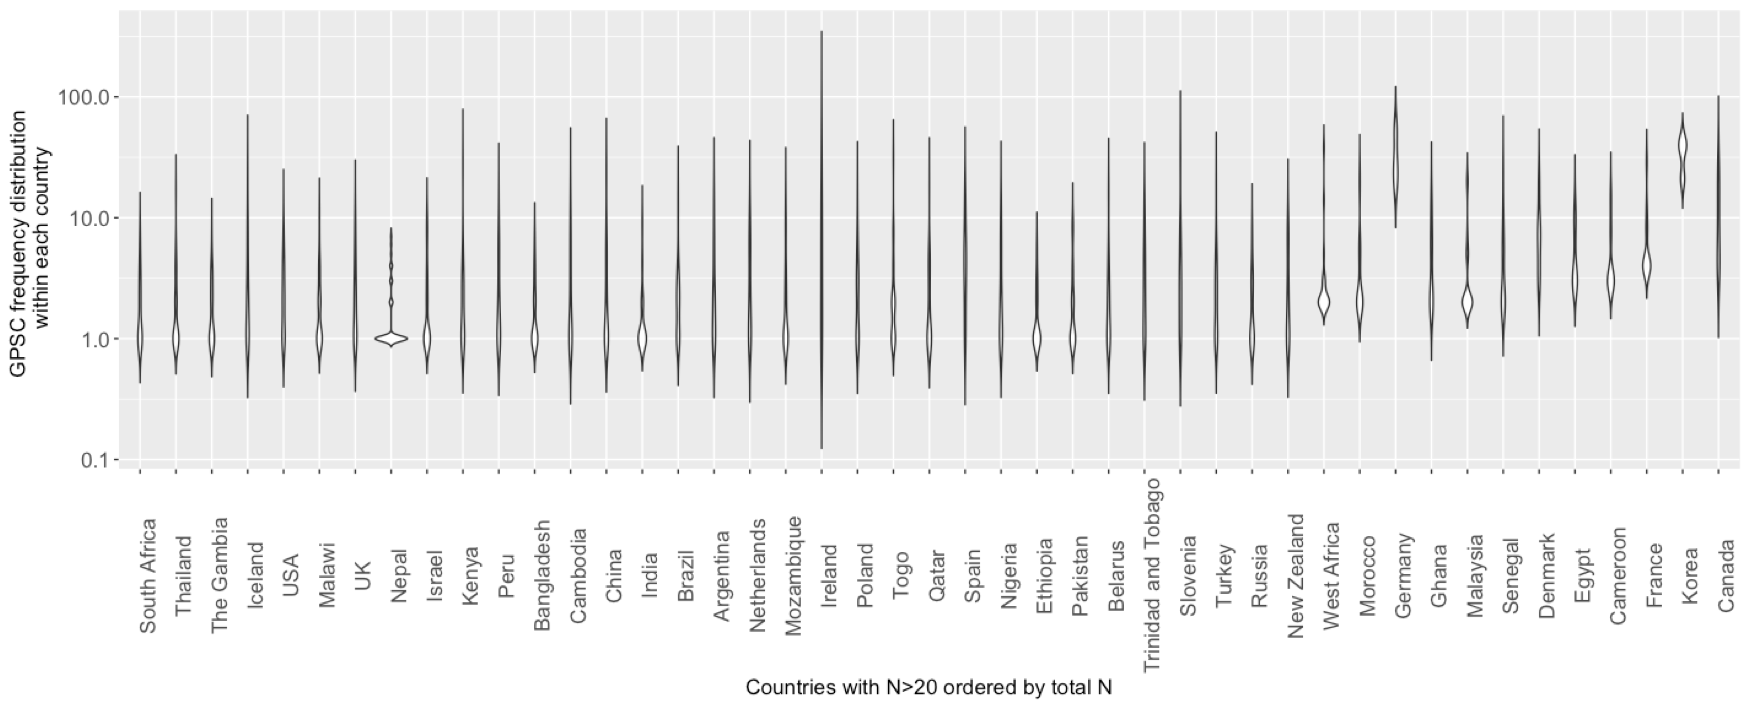
\includegraphics[width=\textwidth]{08MAR21_gpscfreqDistribution.png}
    \caption{Caption}
    \label{fig:gpscfreqdist}
\end{figure} 
Several of these high frequency GPSCs are consistent across countries while low frequency GPSCs are more varied. This may be a result of geographically varied sampling strategies depending upon whether the samples were carriage or disease, the age sampled, co-existing conditions in the individuals being sampled, among other things [PAPERS SHOWING DIFFERENT GPSCS/CCS/SEROTYPES BY AGE DISEASE CARRIAGE ETC].  
\section{Aims}
My PhD is working towards elucidating the spatiotemporal dynamics of the pneumococcus. I began with characterization of an ancient streptococcal genome initially characterized as pneumococcus, with the intention of identifying its closest strain and beginning to understand which strains have persisted for thousands of years and which have recently expanded. 
200 words
\section{Methods}
\subsection{Characteristics of an ancient streptococcal genome}
\subsection{Spatiotemporal dynamics of the pneumococcus in South Africa}
500 words
\section{Results}
1000 words
\section{Discussion}
900 words
\section{Future Work}
1000 words
\section{Gantt Chart}
\printbibliography
\end{document}
